% CSCI 4448
% Spring 2014
% Homework 3: Design Patterns
% Written by Domenic Murtari (3/12/2014)

\documentclass[12pt]{article}

\usepackage[text={6.5in, 9in}, centering]{geometry}
\usepackage{graphicx}
\usepackage{url}

\title{CSCI 4448: Homework 4 \\ Design Patterns}
\author{
  Domenic Murtari \\
  Collaborated with Irakli Zhuzhunashvili and Sean Callahan
}
\date{3/13/2014}

\begin{document}

\maketitle

\section{Structural Problems}
\subsection{Structural Problem 3: Decorator}

Structural Problem 3 gives the description of a Mario character who starts as
a plain, small Mario, and can pick up various power-ups. The decorator pattern 
is most applicable for this application, since the desire is to have a base 
character (the plain Mario), and to be able to customize that Mario by giving
him power-ups.

\begin{figure}[!htb]
  \begin{center}
    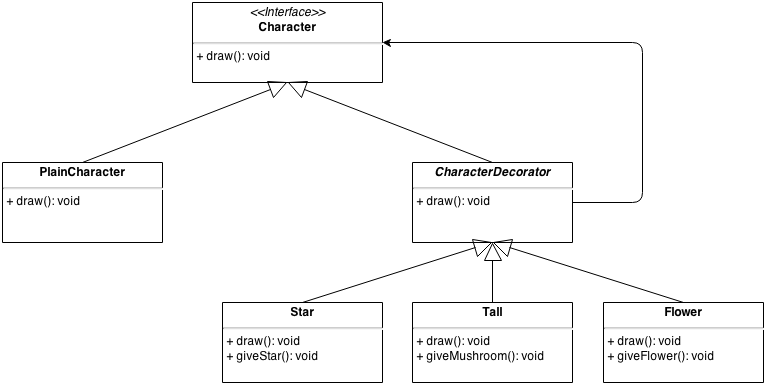
\includegraphics[width=100mm]{Decorator.png}
    \caption{Class diagram of Decorator pattern implementation}
    \label{fig:decorator}
  \end{center} 
\end{figure}

\begin{itemize}
\item Component interface is implemented by {\ttfamily Character}.
\item The concrete component is implemented by {\ttfamily PlainCharacter}.
\item The decorator component which provides the ability to decorate Mario with
  different states of being powered up is implemented by 
  {\ttfamily CharacterDecorator}.
\item The different concrete decorators which provide the ability to add 
  different power-ups to the plain Mario are provided by {\ttfamily Star, Tall} 
  and {\ttfamily Flower}.
\end{itemize}

\newpage
\subsection{Structural Problem 5: Proxy}

Structural Problem 5 describes a bank that needs to access an SQL database, but
would like the commands for the SQL database to be executed after the database
has been closed for the day. The Proxy pattern best solves this problem, because
it allows for the proxy to stand in for the actual database, and the bank will 
issue commands to the proxy which will send the commands to the actual database
once the bank closes for the day.

\begin{figure}[!htb]
  \begin{center}
    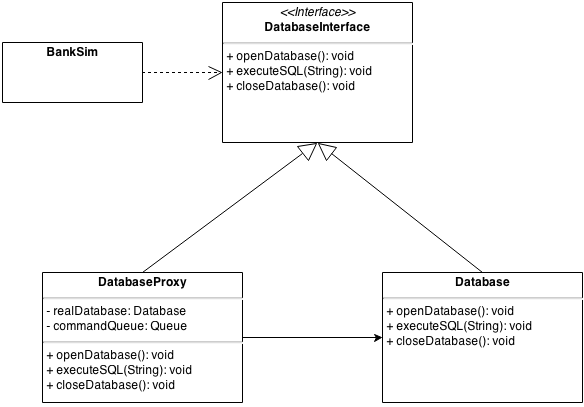
\includegraphics[width=100mm]{Proxy.png}
    \caption{Class diagram of Proxy pattern implementation}
    \label{fig:proxy}
  \end{center} 
\end{figure}

\begin{itemize}
\item The role of the subject interface is played by 
  {\ttfamily DatabaseInterface}, which both the real database and the proxy 
  implement allowing for a consistent interface between the two. 
\item The RealSubject is implemented by {\ttfamily Database} which is the actual 
  instance of the database that the bank interacts with through the proxy.
\item The Proxy is implemented by {\ttfamily Proxy} which allows the bank to
  interact with it as if it were the bank, but issues the SQL commands to the
  real database after the bank closes.
\item The Client is provided by {\ttfamily BankSim} which simulates the bank
  interacting with the database.
\end{itemize}

\newpage
\section{Creational Problems}
\subsection{Creational Problem 1: Singleton}

Creational Problem 1 presents an auto-grader that could potentially be 
multi-threaded, which gives rise to the need for a queue that will be compatible
with multiple threads. The Singleton Pattern solves this, since only one 
singleton can exist (even for multiple threads), and will thus ensure that each
auto-grader running in its own thread will pull from the same queue

\begin{figure}[!htb]
  \begin{center}
    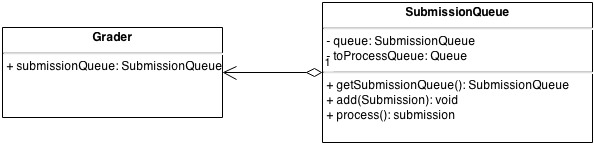
\includegraphics[width=100mm]{Singleton.png}
    \caption{Class diagram of Singleton pattern implementation}
    \label{fig:singleton}
  \end{center} 
\end{figure}

\begin{itemize}
\item The Singleton is represented by {\ttfamily SubmissionQueue}, which 
  maintain a queue of submissions that need to be graded. The constructor for 
  the SubmissionQueue is private, only being invoked by 
  {\ttfamily getSubmissionQueue} which only creates a new 
  {\ttfamily SubmissionQueue} if one does not exist already.
\item The client is represented by {\ttfamily Grader}, which aggregates an
  instance of {\ttfamily SubmissionQueue} and can only instantiate
  SubmissionQueues through the {\ttfamily getSubmissionQueue} method.
\end{itemize}

\newpage
\subsection{Creational Problem 2: Prototype}

Creational Problem 2 gives a neural network that learns. The ability to make new
neural networks without having to have the new neural network relearn everything
that the first neural network learned. The Prototype pattern resolves this 
issue, since the Prototype pattern gives a way for new instances of a class to 
be created which contain information from the original object.

\begin{figure}[!htb]
  \begin{center}
    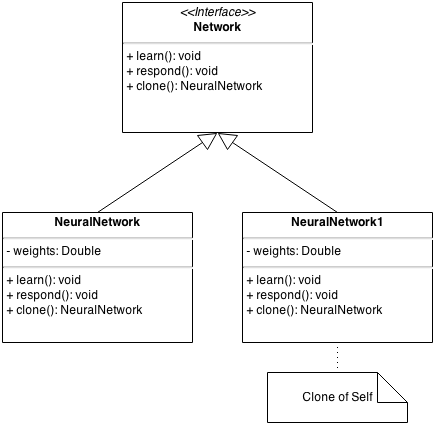
\includegraphics[width=100mm]{Prototype.png}
    \caption{Class diagram of Prototype pattern implementation}
    \label{fig:prototype}
  \end{center} 
\end{figure}

\begin{itemize}
\item The Prototype interface is represented by {\ttfamily Network}, which 
  ensure that any class implementing it will implement a {\ttfamily clone()} 
  method.
\item The Concrete Prototypes are represented by {\ttfamily NeuralNetwork} and
  {\ttfamily NeuralNetwork1}. The client will call {\ttfamily NeuralNetwork}'s 
  {\ttfamily clone()} method, which creates a new neural network object
  {\ttfamily NeuralNetwork1} which contains everything {\ttfamily NeuralNetwork}
  has learned
\end{itemize}

\end{document}